%%%%%%%%%%%%%%%%%%%%%%%%%%%%%%%%%%%%%%%%%
% Arsclassica Article
% LaTeX Template
% Version 1.1 (1/8/17)
%
% This template has been downloaded from:
% http://www.LaTeXTemplates.com
%
% Original author:
% Lorenzo Pantieri (http://www.lorenzopantieri.net) with extensive modifications by:
% Vel (vel@latextemplates.com)
%
% License:
% CC BY-NC-SA 3.0 (http://creativecommons.org/licenses/by-nc-sa/3.0/)
%
%%%%%%%%%%%%%%%%%%%%%%%%%%%%%%%%%%%%%%%%%

%----------------------------------------------------------------------------------------
%	PACKAGES AND OTHER DOCUMENT CONFIGURATIONS
%----------------------------------------------------------------------------------------

\documentclass[
11pt, % Main document font size
a4paper, % Paper type, use 'letterpaper' for US Letter paper
oneside, % One page layout (no page indentation)
%twoside, % Two page layout (page indentation for binding and different headers)
headinclude,footinclude, % Extra spacing for the header and footer
BCOR5mm, % Binding correction
]{scrartcl}
\usepackage{mathrsfs,lipsum,mathptmx,etoolbox} 

%%%%%%%%%%%%%%%%%%%%%%%%%%%%%%%%%%%%%%%%%
% Arsclassica Article
% Structure Specification File
%
% This file has been downloaded from:
% http://www.LaTeXTemplates.com
%
% Original author:
% Lorenzo Pantieri (http://www.lorenzopantieri.net) with extensive modifications by:
% Vel (vel@latextemplates.com)
%
% License:
% CC BY-NC-SA 3.0 (http://creativecommons.org/licenses/by-nc-sa/3.0/)
%
%%%%%%%%%%%%%%%%%%%%%%%%%%%%%%%%%%%%%%%%%

%----------------------------------------------------------------------------------------
%	REQUIRED PACKAGES
%----------------------------------------------------------------------------------------


\usepackage[
nochapters, % Turn off chapters since this is an article        
beramono, % Use the Bera Mono font for monospaced text (\texttt)
pdfspacing, % Makes use of pdftex’ letter spacing capabilities via the microtype package
dottedtoc % Dotted lines leading to the page numbers in the table of contents
]{classicthesis} % The layout is based on the Classic Thesis style

\usepackage{arsclassica} % Modifies the Classic Thesis package

\usepackage[T1]{fontenc} % Use 8-bit encoding that has 256 glyphs

\usepackage[utf8]{inputenc} % Required for including letters with accents

\usepackage{graphicx} % Required for including images
\graphicspath{{Figures/}} % Set the default folder for images

\usepackage{enumitem} % Required for manipulating the whitespace between and within lists
\usepackage{enumerate}

\usepackage{lipsum} % Used for inserting dummy 'Lorem ipsum' text into the template

\usepackage{subfig} % Required for creating figures with multiple parts (subfigures)

\usepackage{amsmath,amssymb,amsthm} % For including math equations, theorems, symbols, etc

\usepackage{varioref} % More descriptive referencing

%----------------------------------------------------------------------------------------
%	THEOREM STYLES
%---------------------------------------------------------------------------------------

\theoremstyle{definition} % Define theorem styles here based on the definition style (used for definitions and examples)
\newtheorem{definition}{Definition}

\theoremstyle{plain} % Define theorem styles here based on the plain style (used for theorems, lemmas, propositions)
\newtheorem{theorem}{Theorem}

\theoremstyle{remark} % Define theorem styles here based on the remark style (used for remarks and notes)

%----------------------------------------------------------------------------------------
%	HYPERLINKS
%---------------------------------------------------------------------------------------

\hypersetup{
%draft, % Uncomment to remove all links (useful for printing in black and white)
colorlinks=true, breaklinks=true, bookmarks=true,bookmarksnumbered,
urlcolor=webbrown, linkcolor=RoyalBlue, citecolor=webgreen, % Link colors
pdftitle={}, % PDF title
pdfauthor={\textcopyright}, % PDF Author
pdfsubject={}, % PDF Subject
pdfkeywords={}, % PDF Keywords
pdfcreator={pdfLaTeX}, % PDF Creator
pdfproducer={LaTeX with hyperref and ClassicThesis} % PDF producer
} % Include the structure.tex file which specified the document structure and layout

\hyphenation{Fortran hy-phen-ation} % Specify custom hyphenation points in words with dashes where you would like hyphenation to occur, or alternatively, don't put any dashes in a word to stop hyphenation altogether

%----------------------------------------------------------------------------------------
%	TITLE AND AUTHOR(S)
%----------------------------------------------------------------------------------------

\title{\normalfontRandom Random Interlacements Essentials and Cover Time of Random Walks} % The article title

%\subtitle{Subtitle} % Uncomment to display a subtitle

\author{Chenxin Gu} % The article author(s) - author affiliations need to be specified in the AUTHOR AFFILIATIONS block

\date{} % An optional date to appear under the author(s)

%----------------------------------------------------------------------------------------

\begin{document}

%----------------------------------------------------------------------------------------
%	HEADERS
%----------------------------------------------------------------------------------------

\renewcommand{\sectionmark}[1]{\markright{\spacedlowsmallcaps{#1}}} % The header for all pages (oneside) or for even pages (twoside)
%\renewcommand{\subsectionmark}[1]{\markright{\thesubsection~#1}} % Uncomment when using the twoside option - this modifies the header on odd pages
\lehead{\mbox{\llap{\small\thepage\kern1em\color{halfgray} \vline}\color{halfgray}\hspace{0.5em}\rightmark\hfil}} % The header style

\pagestyle{scrheadings} % Enable the headers specified in this block

%----------------------------------------------------------------------------------------
%	TABLE OF CONTENTS & LISTS OF FIGURES AND TABLES
%----------------------------------------------------------------------------------------

\maketitle % Print the title/author/date block

\setcounter{tocdepth}{2} % Set the depth of the table of contents to show sections and subsections only

\tableofcontents % Print the table of contents


\let\thefootnote\relax\footnotetext{\textsuperscript{1} \textit{Department of Mathematics, New York University, New York, United States}}

%----------------------------------------------------------------------------------------

\newpage % Start the article content on the second page, remove this if you have a longer abstract that goes onto the second page

%----------------------------------------------------------------------------------------
%	INTRODUCTION
%----------------------------------------------------------------------------------------
\setcounter{section}{-1}
\section{Introduction}
\textit{Random walk} is a stochastic process formed by addition of successive independent, identically distributed random variables. We studied the vacant set left by some random walks on a discrete torus $(\mathbb{Z}/N\mathbb{Z})^d$ until they run up to $uN^d$ time, where $u$ is a non-negative parameter that measures number of trajectories enter into the picture. The model of random interlacements was introduced by A.-S. Sznitman in the seminal paper \cite{sznitman2010vacant}. The aim of this paper was to summarize the basic definitions and properties of random walk and random interlacements and their vacant set following the outline of \cite{drewitz2014introduction}, and also investigate another variation of simple random walk, namely \textit{elephant random walk}.
\vspace{0.6em}\\In chapter $1$, we prepare a series of concepts and theorems for discrete-time stochastic processes that are essential for the discussion of random walks and random interlacements. In chapter $2$, we define simple random walks on $\mathbb{Z}^d$ and look at their key properties. In chapter $3$, we introduce the model of random interlacements and discuss its important trait with respect to discrete lattice shifts. In chapter $4$, we limit our discussion to a discrete torus in $\mathbb{Z}^d$ and we construct a connection between random walks and random interlacements. Finally in chapter $5$, we investigate into elephant random walk and give some conjectures for its cover time.


\section{Some Basic Definitions}
\textbf{Definition 1.1} (Basic concepts for discrete-time stochastic processes).
\begin{itemize}[noitemsep] % [noitemsep] removes whitespace between the items for a compact look
\item A discrete-time real-valued \textit{stochastic process} is a sequence of random variables $X_n:(\Omega, \mathscr{F}) \to (\mathbb{R}, \mathscr{B})$ indexed by $n \in \mathbb{Z}_+$, where $\mathscr{B}$ is the Borel $\sigma$-algebra generated on $\mathbb{R}$. We write such sequences as $(X_n, n \geq 0)$, with the understanding that the time index $n$ is always an integer.
\item A \textit{filtration} is a sequence of sub $\sigma$-algebras $(\mathscr{F}_n, n \geq 0)$ such that $\mathscr{F}_n \subseteq \mathscr{F}_{n+1} \subseteq \mathscr{F}$ for all $n \geq 0$.
\item For a set $K \subset\subset \mathbb{Z}^d$ (cardinality of $K$ is less than $\infty$)
\begin{equation}
    \partial_{ext}K:=\{x \in \mathbb{Z}^d \setminus K \ : \exists y \in K \ s.t. \mid x-y \mid_1=1 \} \tag{1.1}
\end{equation}
is the \textit{exterior boundary} of $K$. Here, $\mid \cdot \mid_1$ denotes the the 1-norm of $\cdot$ in $\mathbb{R}^d$. Any two vertices $x$, $y \in \mathbb{Z}^d$ are called \textit{nearest neighbors} (in $\mathbb{Z}^d$) if $\mid x-y \mid_1=1$. Also,
\begin{equation}
    \partial_{int}K:=\{x \in K \ : \exists y \in \mathbb{Z}^d \setminus K \ s.t.\mid x-y \mid_1=1 \} \tag{1.2} 
\end{equation}
is the \textit{interior boundary} of $K$.
\item A random variable $\tau \in \mathbb{Z}_+\cup \{\infty\}$ is a \textit{stopping time} with respect to a filtration $(\mathscr{F}_n, n \geq 0)$ if $\{\tau=n\} \in \mathscr{F}_n$ for all $n \geq 0$.
\end{itemize}

\textbf{Definition 1.2} (Markov chains).
\begin{itemize}
    \item A process $(X_n)$ is a \textit{Markov chain} on space $A$ which we assume $A$ a countable set, take any $n \geq 0$ and $m \geq 1$,
\begin{equation}
\mathbf{P} [X_{n+m}=y \mid X_0, \dots X_n]=\mathbf{P}[X_{n+m}=y \mid X_n]\ a.s. \tag{1.3}
\end{equation}
In words, a Markov chain is a stochastic process such that the probability for it to transit into any future state does not require all information about its previous trajectory, but depends solely on its current state.
\item \textit{Strong Markov property:} Let $(X_n)$ be a Markov chain on a countable set $A$ and $\tau$ be a stopping time with respect the the natural filtration of $X_n$, then for all $x, \ y_1, \dots , y_k$, it holds that 
\begin{equation}
\label{SMP}
    \mathbf{P}[X_{\tau +n_j}=y_j,\ j=1,\dots, k \mid \mathscr{F}_\tau, \ X_\tau = x]=\mathbf{P}_x[X_{\tau +n_j}=y_j, \ j=1,\dots,k] \tag{1.4}
\end{equation}
\end{itemize}
\section{Random Walks}
In terminology of \cite{drewitz2014introduction}, we first define simple random walk and discuss its properties. 
\subsection{Simple Random Walk}
Consider the measurable space $(\overline{RW}$, $\overline{\mathscr{RW}})$, where $\overline{RW}$ is the set of infinite $\mathbb{Z}^d$-valued sequences $w = (w_n)_{n \geq 0}$ and $\overline{\mathscr{RW}}$ is the $\sigma$-algebra generated on $\overline{RW}$ by coordinate maps $X_n : \overline{RW} \to \mathbb{Z}^d$, $X_n(w)=w_n$. 
\\For $x \in \mathbb{Z}^d$, we consider the probability measure $\mathbf{P}_x$ on $(\overline{RW}$, $\overline{\mathscr{RW}})$ such that under $\mathbf{P}_x$, the random sequence $(X_n)_{n \geq 0}$ is a Markov chain on $\mathbb{Z}^d$ that starts at $x$ and has transition probabilities
\begin{equation}
\mathbf{P}_x[X_{n+1}=y' \mid X_n=y]:=\left\{
\begin{aligned}
\frac{1}{2d}, & \quad if \mid y-y' \mid_1 =1\\
0, & \quad otherwise
\end{aligned}
\right.\tag{2.1}
\end{equation}
\begin{figure}[htb]
    \centering
    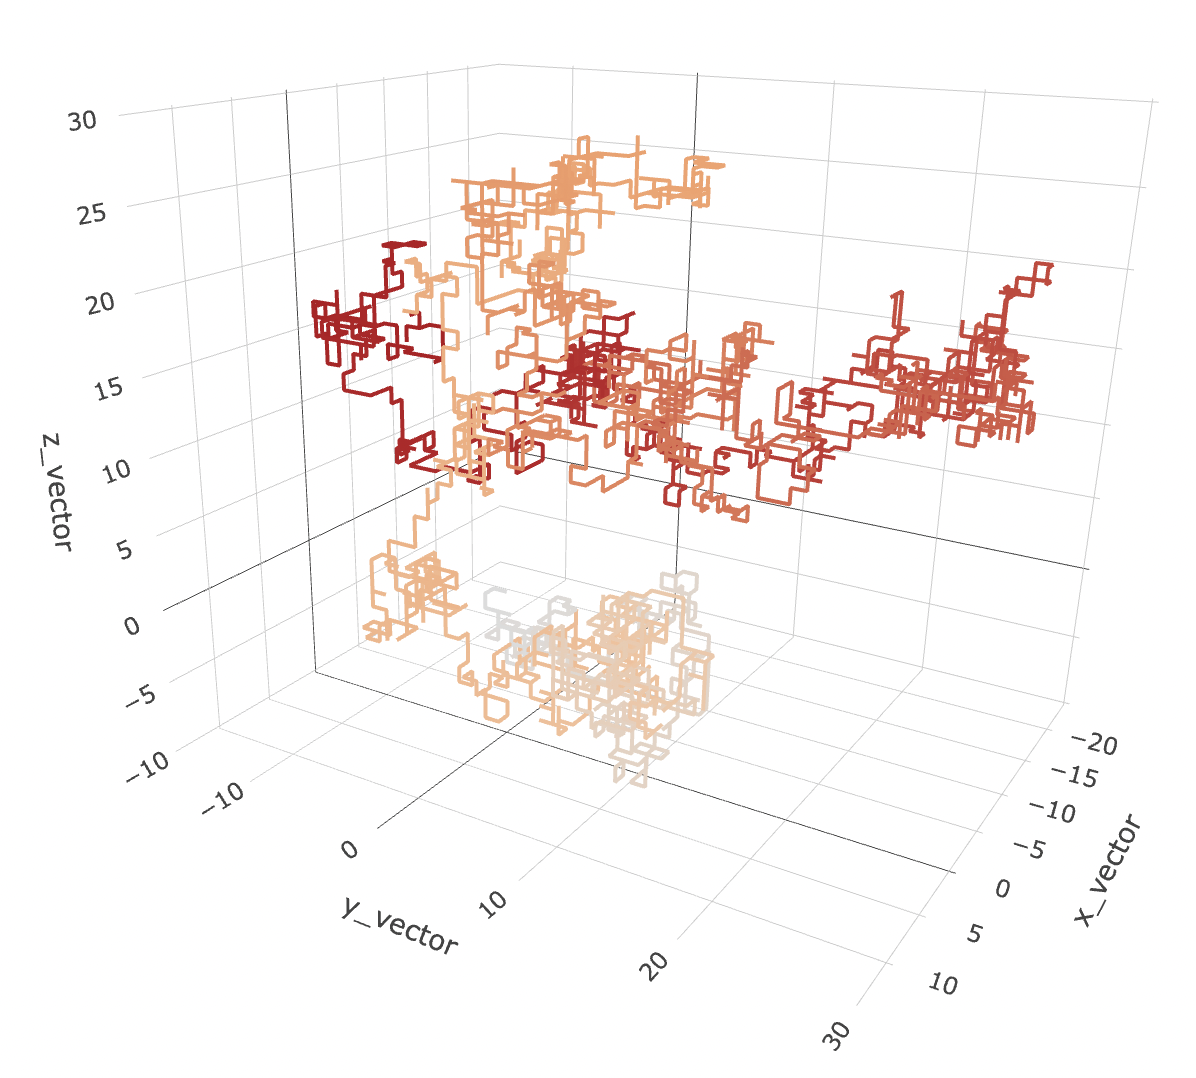
\includegraphics[width=.6\columnwidth]{Figures/3d rw fixed.png}
    \caption{Simple Random Walk on Three Dimensions}
    \label{3dSRW}
\end{figure}
for all $y$, $y' \in \mathbb{Z}^d$. In words, $X_{n+1}$ has the uniform distribution over the nearest neighbors of $X_n$ and reaches other vertices at zero probability. The random sequence $(X_n)_{n \geq 0}$ on $(\overline{RW}$, $\overline{\mathscr{RW}}$, $\mathbf{P})$ is called \textit{simple random walk} (SRW) on $\mathbb{Z}^d$ starting in $x$. An example of a simple random walk in three dimensions is shown in Figure~\ref{3dSRW}, in which the color change represents time change respectively.

Now we define several key random times that are essential to our following discussion.
\vspace{0.6em}\\\textbf{Definition 2.1.1}\ (entrance time, hitting time, exit time, last visit time). For any $A \subseteq \mathbb{Z}^d$,
\begin{itemize}
    \item First entrance time:
    \begin{equation}
    \label{eq2.2}
    H_A(w):= \inf \{n \geq 0:X_n(w) \in A\}\tag{2.2} 
    \end{equation}
    \item First hitting time:
    \begin{equation}
    \Tilde{H}_A(w):=\inf\{n \geq 1:X_n(w) \in A\}\tag{2.3}
    \end{equation}
    \item First exit time:
    \begin{equation}
    T_A(w):=\inf\{n \geq 0:X_n(w) \notin A \}\tag{2.4}
    \end{equation}
    \item Last visit time:
    \begin{equation}
    L_A(w):=\sup\{ n \geq 0:X_n(w) \in A \}\tag{2.5}
    \end{equation}   
\end{itemize}
\textit{Remark 2.1}\ If a random walk starts in $\partial_{int}K$ and leaves the set $K$, i.e. $X_0(w) \in \partial_{int}K$ and $X_1(w) \in \partial_{ext}K$, and it enters the set again at time $\Tilde{t}$, its first entrance time $H_A(w)$ will be $0$, while its first hitting time $\Tilde{H}_A(w)$ will be $\Tilde{t}$. 
\vspace{0.6em}\\\textit{Remark 2.2}\ $H_A$ is a stopping time with respect to the canonical filtration $\mathscr{F}_n$ since 
\begin{equation}
    \label{eqstoppingtime}
    \begin{aligned}
    \{H_A=n\}&=\{X_0 \notin K\} \cap \{X_1\notin K\} \cap \dots \cap \{X_{n-1}\notin K\} \cap \{X_n\in K\}\\
    &\in \sigma(\{X_0, \ X_1, \dots , \ X_n\})
    \end{aligned}\notag
\end{equation}
By similar proof, one can easily check that $\Tilde{H}_A$, and $T_A$ are also stopping times with respect to $\mathscr{F}_n$. 
\subsection{Green function}
\textbf{Definition 2.2.1}\ (Green function) The \textit{Green function} of a simple random walk on $\mathbb{Z}^d$ is defined as
\begin{equation}
    g(x,\ y)=\sum_{n \geq 0}\mathbf{P}_x[X_n=y]=\mathbf{E}_x\left[\sum_{n \geq 0} \mathbb{1}_{\{X_n=y\}}\right], \ x, y \in \mathbb{Z}^d.\tag{2.6}
\end{equation}
\textit{Remark 2.3}\ By our definition, $g(x,\ x)>1$ in all dimensions. Informally speaking, in the case $x=y$, we still count it as one visit.
The Green function measures the expected number of visits of a SRW to $y$ if it starts in $x$. By symmetry and translation invariance, it holds that $g(x,\ y)=g(y, \ x)=g(0,\ y-x)$. Thus we use the notation $g(x):=g(0,x)$ for simplicity. 
\vspace{0.6em}\\The notion of Green function is closely related to an essential notion of SRW, normally that of transience and recurrence.
\vspace{0.6em}\\\textbf{Definition 2.2.2}\ A simple random walk is \textit{transient} if $\mathbf{P}_0[\Tilde{H}_0=\infty]>0$, and is called \textit{recurrent} otherwise. 
\vspace{0.6em}\\In words, a simple random walk is transient if it has positive probability to never return to its starting location, otherwise it is recurrent. Here we introduce a fundamental theorem of SRWs on integer lattices from George Pólya's result in \cite{polya1921aufgabe}.
\vspace{0.6em}\\\textbf{Theorem 2.1}\ \textit{SRW on} $\mathbb{Z}^d$ \textit{is recurrent if} $d \leq 2$ \textit{and transient if} $d>2$.
\vspace{0.6em}\\In order to understand the notions of transience and recurrence better, we check one of the properties of the Green function. 
\vspace{0.6em}\\\textbf{Lemma 2.1}\ $g(0)=\mathbf{P}_0[\Tilde{H}_0=\infty]^{-1}$, in particular, SRW is transient if and only if $g(0)<\infty$.
\begin{proof}
    The main idea is to employ \textit{the last-visit decomposition}. For a set $K \subset\subset \mathbb{Z}^d$, for $i \in \mathbb{N}$, we denote $\theta_i(w)$ to be a segment of the random walk that starts at time $t=i$. Also, let $H_K^{(i)}$ be the $i$-th entrance of the random walk into the set $K$. By using this notation, we can decompose entrance time and exit time. Thus,
    \begin{equation}
        \Tilde{H}_K^{(k)}=\Tilde{H}_K^{(k-1)}+\Tilde{H}_K \circ \theta_{\Tilde{H}_K^{(k-1)}}, \ k \geq 2.\tag{2.7}
    \end{equation}
    We first consider the case when $d \leq 2$. Using Theorem 2.1, we know SRW is recurrent, thus
    \begin{equation}
        \mathbf{P}[\Tilde{H}_0= \infty]=0. \tag{2.8}
    \end{equation}
    It suffices to prove
    \begin{equation} g(0)=\sum^\infty_{n=0}\mathbf{P}_0[X_n=0]=\mathbf{E}_0\left[\sum^\infty_{n=0} \mathbb{1}_{\{X_n=0\}}\right]=\infty.\tag{2.9}
    \end{equation}
    Applying strong Markov property as stated in \ref{SMP}, we can deduce 
    \begin{align}
        \mathbf{P}_0[\Tilde{H}_0^{(2)}<\infty]&=\mathbf{P}_0[\Tilde{H}_0^{(1)}<\infty, \ \Tilde{H}_0^{(1)} + \Tilde{H}_0 \circ \theta_{\Tilde{H}_0^{(1)}}<\infty] \notag \\ 
        &=\mathbf{P}_0[\Tilde{H}_0<\infty, \ \Tilde{H}_0 \circ \theta_{\Tilde{H}_0}<\infty] \notag \\
        &=\mathbf{E}_0\left[\mathbb{1}_{\{\Tilde{H}_0<\infty, \ \Tilde{H}_0 \circ \theta_{\Tilde{H}_0}<\infty\} }\right] \notag \\ 
        &=\mathbf{E}_0 \left[ \mathbf{E}_0 [ \mathbb{1}_{\{\Tilde{H}_0<\infty, \ \Tilde{H}_0 \circ \theta_{\Tilde{H}_0}<\infty\} } \mid \mathscr{F}_{\Tilde{H}_0} ] \right] \notag \\ 
        &=\mathbf{E}_0 \left[ \Tilde{H}_0<\infty, \ \mathbf{E}_{X_{\Tilde{H}_0}} [ \mathbb{1}_{{\Tilde{H}_0<\infty}} ] \right]. \notag 
    \end{align}
    Note that $\mathbf{E}_{X_{\Tilde{H}_0}} [ \mathbb{1}_{{\Tilde{H}_0<\infty}} ]=\mathbf{P}_0[\Tilde{H}_0<\infty]=1$, we know 
    \begin{equation}
        \mathbf{P}_0[\Tilde{H}_0^{(2)}<\infty]=\mathbf{P}_0[\Tilde{H}_0<\infty]=1. \tag{2.10}
    \end{equation}
    By mathematical induction, we conclude $\Tilde{H}_0<\infty$, $\Tilde{H}_0^{(2)}<\infty$, $\Tilde{H}_0^{(3)}<\infty$,$\dots$, $\Tilde{H}_0^{(n)}<\infty$ $\mathbf{P}_0$-almost surely. So,
    \begin{equation}
        \sum^\infty_{n=0} \mathbb{1}_{\{X_n=0\}}=\sum^\infty_{k=1} \mathbb{1}_{\{\Tilde{H}^{(k)}_0<\infty\}}+1 \quad \mathbf{P}_0 \text{ - a.s.} \tag{2.11}
    \end{equation}
    \begin{equation}
        \sum^\infty_{k=1} \mathbb{1}_{\{\Tilde{H}^{(k)}_0<\infty\}} \rightarrow \infty \quad \mathbf{P}_0 \text{ - a.s.}\tag{2.12}
    \end{equation}
    Thus we conclude $g(0)= \infty$.
    \\Now we prove the other direction, consider the transient case. Again using \eqref{SMP}, we get
    \begin{align}
        \mathbf{P}_0 \left[ \sum^\infty_{k=1} \mathbb{1}_{ \{ H_0^{(k)}<\infty\} }=n \right]&=\mathbf{P}_0 \left[ H_0^{(1)}<\infty, \ H_0^{(2)}<\infty, \dots, H_0^{(n)}<\infty, \ H_0^{(n+1)}=\infty \right] \notag \\
        &=\mathbf{E}_0 \left[ \mathbf{E}_0 \left[ \mathbb{1}_{ \{H_0^{(1)}<\infty, \dots, H_0^{(n)}<\infty, \ H_0^{(n+1)}=\infty\} }\right]\right] \notag \\
        &=\mathbf{E}_0 \left[ \mathbf{E}_0 \left[ \mathbb{1}_{ \{H_0^{(1)}< \infty, \dots, H_0^{(n)}<\infty \}} \cdot \mathbb{1}_{ \{ \Tilde{H}_0^{(n+1)}=\infty \} } \circ \theta_{H_0^{(n)}} \mid \mathscr{F}_{H_0^{(n)}} \right] \right] \notag \\
        &=\mathbf{P}_0[\Tilde{H}_0=\infty] \cdot \mathbf{P}_0[H_0^{(1)}<\infty, \dots, H_0^{(n)}<\infty] \notag \\
        &=\mathbf{P}_0[\Tilde{H}_0=\infty] \cdot (1-\mathbf{P}_0[\Tilde{H}_0=\infty]). \notag
    \end{align}
Note that 
    \begin{equation}
        \sum^\infty_{k=1} \mathbb{1}_{ \{ H_0^{(k)}<\infty\} } \sim Geom(\mathbf{P}_0[\Tilde{H}_0=\infty]).\tag{2.13}
    \end{equation}
    \begin{equation}
        g(0)=\mathbf{E}_0\left[ \sum^\infty_{n=0} \mathbb{1}_{\{X_n=0\}}\right] =\mathbf{E}_0 \left[ \sum^\infty_{k=1} \mathbb{1}_{\{H^{(k)}_0<\infty\}}+1 \right]=\frac{1}{\mathbf{P}_0[\Tilde{H}_0=\infty]}<\infty.\tag{2.14}
    \end{equation}
\end{proof}

\subsection{Equilibrium Measure and Capacity}
We now focus on the case when dimension $d$ is greater or equal to three, i.e. the random walk is transient. Fix a set $K \subset\subset \mathbb{Z}^d$ and $x \in \mathbb{Z}^d$, we can define the equilibrium measure and the capacity of $K$.
\vspace{0.6em}\\\textbf{Definition 2.3.1}\ (equlibrium measure) For $K \subset\subset \mathbb{Z}^d$ and $x \in \mathbb{Z}^d$, 
\begin{equation}
    e_K(x):=\mathbf{P}_x[\Tilde{H}_K=\infty]\cdot \mathbb{1}_{x \in K}=\mathbf{P}_x[L_K=0]\cdot \mathbb{1}_{x \in K}. \tag{2.15}
\end{equation}
\textbf{Definition 2.3.2}\ (capacity) The total mass of $e_K(x)$ for all $x \in K$ is called the \textit{capacity} of $K$.
\begin{equation}
    cap(K):=\sum_{x \in K} e_K(x)=e_K(K)=e_K(\mathbb{Z}^d). \tag{2.16}
\end{equation}    
Intuitively, $e_K(x)$ is not trivial when $x$ lives in the interior boundary of $K$, $\partial_{int} K$. The following definition of normalized equilibrium measure gives us a probability measure on $K$.
\vspace{0.6em}\\\textbf{Definition 2.3.3}\ (normalized equilibrium measure, also "harmonic measure" with respect to $K$) For any $K \subset\subset \mathbb{Z}^d$ and $K \neq \varnothing$, 
\begin{equation}
    \label{eq3.11}
    \Tilde{e}_K(x):=\frac{e_K(x)}{cap(K)}. \tag{2.17} 
\end{equation}   
For more properties about simple random walk on $\mathbb{Z}^d$, one could read Lawler's book \cite{lawler2013intersections}.
\subsection{Lazy Random Walks}
One more definition that will be essential to proof in Chapter $4$ is that of \textit{lazy random walks}, slightly modified from simple random walks. Simple random walks are periodic due to their construction. In fact, $(X_{2i+1})$ and $(X_{2i})$ will be disjoint subsets of $\mathbb{Z}^d$, $i \in \mathbb{N}_0$. The lazy random walk $(Y_n)_{n \geq 0}$ is defined as the Markov chain which has probability $0.5$ to stay in its current state. Thus, conditionally on $\{Y_n = y_n\}$, $y_n \in \mathbb{Z}^d$,
\begin{equation}
Y_{n+1} =\left\{
\begin{aligned}
y_n + e_i, & \quad \text{at probability } \frac{1}{4}\\
y_n - e_i, & \quad \text{at probability } \frac{1}{4}\\
y_n, & \quad \text{at probability } \frac{1}{2}
\end{aligned}
\right.\tag{2.18}
\end{equation}
where $e_i$ is selected uniformly at random from the standard basis of $\mathbb{Z}^d$, namely $\left(e_i\right)_{i=i}^d$. 
\vspace{0.6em}\\ It's also beneficial to construct lazy random walks directly from simple random walks. Define the sequence of $(\xi_n)_{n \geq 1}$ to be i.i.d random variables such that $\xi_n \sim Ber(\frac{1}{2})$ with values in $\{0,1\}$ independent of $(X_n)$. Then, let $S_0=0$, $S_n=\sum_{i=1}^n\xi_i$ for $n \geq 1$. $Y_n := X_{S_t}$ is the induced lazy random walk where $S_n$ traces the number of steps when the walk changes it position.
\vspace{0.6em}\\ The aim of introducing the concept of lazy random walks is to avoid periodicity of simple random walk. An important property of the lazy random walk is its aperiodicity, starting from any position converges to the uniform measure on vertices of $(\mathbb{Z}/N\mathbb{Z})^d$. By the law of large numbers, a lazy random walk changes its position about $\frac{n}{2}$ times as $n \rightarrow \infty$. We will further discuss that in Chapter 4.
\section{Random Interlacements: Basic Definitions and Properties}
We will start by introducing the random interlacement model in high dimensions $(d \geq 3)$ at level $u>0$ as a random subset of $\mathbb{Z}^d$. Random interlacement in two dimensions are defined differently due to recurrence of SRW on two dimensions by Theorem 2.1.
\subsection{Space of Subsets of $\mathbb{Z}^d$}
In order to define random interlacements, we first need to put the one-to-one correspondence between the space $\{0,1\}^{\mathbb{Z}^d}(d \geq 3)$ and the subsets of $\mathbb{Z}^d$ in words. For every $\xi \in \{0,1\}^{\mathbb{Z}^d}$, the corresponding subset of $\mathbb{Z}^d$ is defined by
\begin{equation}
    \mathscr{I}(\xi)=\{ x \in \mathbb{Z}^d: \ \xi_x=1 \}. \notag
\end{equation}
\begin{figure}[htb]
\centering 
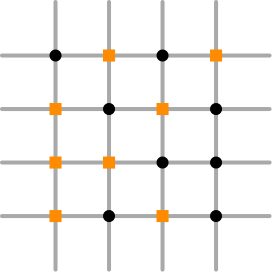
\includegraphics[width=0.3\columnwidth]{Figures/coordinate map.png} 
\caption[coordinate map]{An example of an element in $\{0,1\}^{\mathbb{Z}^2}$} 
\label{coordinate map} 
\end{figure}
The process is to construct a configuration by randomly assigning zeros and ones to each element of $\mathbb{Z}^d$. A concrete example for a $\xi$ in $\{0,1\}^{\mathbb{Z}^2}$ could be like Figure~\ref{coordinate map}, where orange squares stand for "$1$" and black dots stand for "$0$". Thus we can then define coordinate maps, local event and cylinder events.
\vspace{0.6em}\\\textbf{Definition 3.1.1}\ (coordinate map) Consider the space $\{0,1\}^{\mathbb{Z}^d}$ as the space of subsets of $\mathbb{Z}^d$. For $x\in \mathbb{Z}^d$ and $\xi \in \{0,1\}^{\mathbb{Z}^d}$, the functions
\begin{align}
    &\psi_x: \ \{0,1\}^{\mathbb{Z}^d} \rightarrow \{0,1\} \notag \\
    &\psi_x(\xi)=\xi_x \notag
\end{align}
are called \textit{coordinate maps}.
\vspace{0.6em}\\\textbf{Definition 3.1.2}\ (local event, cylinder event) For $K \subset \mathbb{Z}^d$, we denote by $\sigma(\psi_x, \ x \in K)$ the sigma-algebra on the space $\{0,1\}^{\mathbb{Z}^d}$ generated by the coordinate maps $\psi_x, \ x \in K$, and we define $\mathscr{F}_K=\sigma(\psi_x, \ x \in K)$.
\\If $K \subset\subset \mathbb{Z}^d$ and $A \in \sigma(\psi_x, \ x \in K)$, then we say that $A$ is a \textit{local event} with support $K$.
\\For any $K_0 \subseteq K \subset\subset \mathbb{Z}^d$, $K_1=K\setminus K_0$, we say that
\begin{equation}
    \label{eq3.1}
    \{\forall x \in K_0: \ \psi_x=0; \ \forall x \in K_1: \ \psi_x=1\}=\{\mathscr{I} \cap K=K_1\} \tag{3.1}
\end{equation}
is a \textit{cylinder event} with base $K$.
\vspace{0.6em}\\\textit{Remark 3.1} The events $\{\psi_x=1\}$, $x \in \mathbb{Z}^d$ could be considered as "building blocks" of any local event. A local event with support $K$ does not require every $x \in K$ to be mapped, but a cylinder event with base $K$ precisely assigns every $x \in K$ by $\psi_x$ to either $0$ or $1$. Thus, every local event is a finite disjoint union of cylinder events. For any $K \subset\subset \mathbb{Z}^d$, the sigma-algebra generated on $\psi_x$ is atomic and has exactly $2^{\mid K \mid}$ atoms of form \eqref{eq3.1}.
\vspace{0.6em}\\\textit{Example 3.1} Consider $K=\{ (0,0), (0,1),  (1,0),  (1,1) \}$ and the local event $A=\{ \psi_{(0,0)}=1, \psi_{(1,0)}=0\} \in \sigma(\psi_x,x \in K)$, we want to represent this event by cylinder events. Notice that $(1,1)$ and $(0,1)$ are not mapped to a specific value,
\begin{align}
A &=\left\{ \psi_{(0,0)}=1, \psi_{(1,0)}=0\right\} \cap \left( \left\{         \psi_{(0,1)}=1, \psi_{(1,1)}=1\right\}\right.\notag \\ 
    &\quad \cup \left\{ \psi_{(0,1)}=1, \psi_{(1,1)}=0\right\} \cup \left\{ \psi_{(0,1)}=0, \psi_{(1,1)}=1\right\} \notag \\
    &\left. \quad \cup \left\{ \psi_{(0,1)}=0, \psi_{(1,1)}=0\right\} \right) \notag \\
    &=\left\{\psi_{(0,0)}=1, \psi_{(1,0)}=0,\psi_{(0,1)}=1, \psi_{(1,1)}=1 \right\} \notag \\
    &\quad \cup \left\{\psi_{(0,0)}=1, \psi_{(1,0)}=0,\psi_{(0,1)}=0, \psi_{(1,1)}=1 \right\}\notag \\
    &\quad  \cup \left\{\psi_{(0,0)}=1, \psi_{(1,0)}=0,\psi_{(0,1)}=1, \psi_{(1,1)}=0 \right\} \notag \\
    &\quad \cup \left\{\psi_{(0,0)}=1, \psi_{(1,0)}=0,\psi_{(0,1)}=0, \psi_{(1,1)}=0 \right\}. \notag 
\end{align}
Clearly, $A$ can be expressed explicitly as a disjoint union of cylinder events. Based on such a map, we are now able to discuss the law that brings up the definition of random interlacements.
\subsection{Random Interlacements}
\textbf{Definition 3.2.1}\ (random interlacements) For $u>0$, we consider the one-parameter family of probability measures $\mathscr{P}^u$ on $(\{0,1\}^{\mathbb{Z}^d}, \ \mathscr{F})$ such that
\begin{equation}
    \label{eq3.2}
    \mathscr{P}^u[\mathscr{I} \cap K=\varnothing]=e^{-u\text{cap}(K)}. \tag{3.2}
\end{equation}
A random subset $\mathscr{I}$ of $\mathbb{Z}^d$ in $(\{0,1\}^{\mathbb{Z}^d}, \ \mathscr{F}, \ \mathscr{P}^u)$ fulfills \eqref{eq3.2} is called \textit{random interlacements} at level $u$.
\vspace{0.6em}\\\textit{Remark 3.2} The existence of the probability measure $\mathscr{P}^u$ is not obvious. The important idea that we also employed in later simulation is, the measure $\mathscr{P}^u$ also arises as the local limit of the trace of the first $\lfloor uN^d \rfloor$ steps of simple random walk with a uniform starting point on the $d$-dimensional torus $(\mathbb{Z}/N\mathbb{Z})^d$. One can formulate that construction by employing a random interlacement point process for segments of trajectories. Namely, it is a process of randomly dropping segments of trajectories into the space of a discrete torus.
\vspace{0.6em}\\The explicit expression for the probabilities of cylinder evensts is given by: for any $K_0 \subseteq K \subset\subset \mathbb{Z}^d$, $K_1=K \setminus K_0$,
\begin{equation}
    \mathscr{P}^u[\psi \mid_{K_0} \equiv 0, \psi \mid_{K_1} \equiv 1]=\mathscr{P}^u[\mathscr{I} \cap K=K_1]=\sum_{K' \subseteq K_1}(-1)^{\mid K' \mid}e^{-u\text{cap}(K_0 \cup K')}. \tag{3.3}
\end{equation}
\begin{proof}
    The idea is to use the inclusion-exclusion formula. Indeed,
    \begin{align}
        \{\mathscr{I} \cap K=K_1\}&=\{ \mathscr{I} \cap K_0 = \varnothing \} \cap \bigcap_{x \in K_1}\{ \mathscr{I} \cap \{x \} = \varnothing \}^c \notag \\
        &=\{ \mathscr{I} \cap K_0= \varnothing\}\setminus\left(\bigcup_{x \in K_1}\{ \mathscr{I} \cap \{x\} = \varnothing\}\right). \notag
    \end{align}
    Thus,
    \begin{align}\
        \label{eq3.4}
        \mathscr{P}^u[\{\mathscr{I} \cap K=K_1]&=\mathscr{P}^u\left[\{ \mathscr{I} \cap K_0= \varnothing\}\setminus\left(\bigcup_{x \in K_1}\{ \mathscr{I} \cap \{x\} = \varnothing\}\right)\right] \notag \\
        &=\mathscr{P}^u[\mathscr{I} \cap K_0= \varnothing] - \notag \\ & \quad \mathscr{P}^u \left[ \{ \mathscr{I} \cap K_0= \varnothing\} \cap \left(\bigcup_{x \in K_1}\{ \mathscr{I} \cap \{x\} = \varnothing\}\right) \right] \notag \\
        &=\mathscr{P}^u[\mathscr{I} \cap K_0= \varnothing] - \notag \\ & \quad \mathscr{P}^u \left[ \bigcup_{x \in K_1}\{ \mathscr{I} \cap (K_0 \cup \{x\}) = \varnothing \} \right]. \tag{3.4} 
    \end{align}
    Here we can employ the inclusion-exclusion formula,
    \begin{align}
        \label{eq3.5}
        &\mathscr{P}^u \left[ \bigcup_{x \in K_1}\{ \mathscr{I} \cap (K_0 \cup \{x\}) = \varnothing \} \right] \notag \\
        =&\sum_{J \neq \varnothing \subseteq K_1}(-1)^{\mid J \mid + 1} \cdot \mathscr{P}^u \left[ \bigcap_{x \in J}\{ \mathscr{I} \cap (K_0 \cup \{x\}) = \varnothing \} \right] \notag \\
        =&\sum_{J \neq \varnothing \subseteq K_1}(-1)^{\mid J \mid + 1} \cdot \mathscr{P}^u[\mathscr{I} \cap (K_0 \cup J) = \varnothing]. \tag{3.5}
    \end{align}
    Thus from \eqref{eq3.4}, we get
    \begin{align}
        \label{eq3.6}
        \mathscr{P}^u[\mathscr{I} \cap K=K_1]&=e^{-u \text{cap}(K_0)} + \sum_{\varnothing \neq K' \subseteq K_1} (-1)^{\mid K' \mid}e^{-u \text{cap}(K_0 \cup K')} \notag \\
        &=\sum_{K' \subseteq K_1}(-1)^{\mid K \mid}e^{-u \text{cap}(K_0 \cup K')}. \tag{3.6}
    \end{align}   
\end{proof}
\subsection{Ergodicity}
In this section, we will explore the behavior of random interlacements under transformation. Finally, it is important to see that RI is ergodic with respect to lattice shifts. For completeness, we recall the definition of measurability.
\vspace{0.6em}\\\textbf{Definition 3.3.1}\ (measurable) A transformation $T:\ (\Omega,\mathscr{F}) \rightarrow (\Omega,\mathscr{F})$ is \textit{measurable} if for any measurable set $A \in \mathscr{F}$, the preimage is again measurable, that is $T^{-1}(A) \in \mathscr{F}$.
\vspace{0.6em}\\\textbf{Definition 3.3.2}\ (measure preserving) Let $\mathbf{P}$ be a probability measure on $(\Omega, \mathscr{F})$. A \textit{measure-preserving transformation} $T$ on $(\Omega, \mathscr{F}, \mathbf{P})$ is an $\mathscr{F}$-measurable map $T: \ (\Omega,\mathscr{F}) \rightarrow (\Omega,\mathscr{F})$ such that
\begin{equation}
    \label{eq3.7}
    \mathbf{P}[T^{-1}(A)]=\mathbf{P}[A] \text{ for all }A \in \mathscr{F}. \tag{3.7}
\end{equation}
We also say that the transformation $T$ preserves $\mathbf{P}$. If $\mathbf{P}$ satisfies \eqref{eq3.7}, we also say that the measure $\mathbf{P}$ is \textit{invariant} under the transformation $T$. Such a measure-preserving transformation is called \textit{ergodic} if all $T$-invariant events (i.e.~events $A \in \mathscr{F}$ for which $T^{-1}(A) = A$), have $\mathbf{P}$-probability $0$ or $1$.
\\Now we want to consider the measure-preserving transformation $t_x$ on \\
$(\{0,1\}^{\mathbb{Z}^d},\mathscr{F},\mathscr{P}^u)$ called canonical shift. RI under such transformation is ergodic. Ergodicity is important for us to further restrict our discussion on a finite subset in $\mathbb{Z}^d$ because it could be informally considered as a weaker statement of independence. 
\vspace{0.6em}\\\textbf{Definition 3.3.3}\ (canonical shift) A \textit{canonical shift} is defined as 
\begin{align}
    &t_x: \ \{0,1\}^{\mathbb{Z}^d} \rightarrow \{0,1\}^{\mathbb{Z}^d} \notag \\
    &\psi_y(t_x(\xi))=\psi_{y+x}(\xi), \quad y \in \mathbb{Z}^d, \ \xi \in \{0,1\}^{\mathbb{Z}^d}. \notag
\end{align}
Also, for $K \subseteq \mathbb{Z}^d$, $K+x=\{ y+x: \ y \in K \}$. It holds for any $x \in \mathbb{Z}^d$ and for any $u>0$, the transformation $t_x$ preserves the measure $\mathscr{P}^u$. Indeed, one can check this statement first for cylinder events depending on finitely many coordinates, and use standard arguments from measure theory (the \textit{Dynkin-$\pi$-$\lambda$-theorem}) to extend it to all events. We refer to~\cite[Lemma 2.8]{drewitz2014introduction} for details. Finally, we reach the most essential theorem of this section, stating that random interlacements is ergodic with respect to the canonical shifts.
\vspace{0.6em}\\\textbf{Theorem 3.1}\ \textit{For any }$u \geq 0$ \textit{and} $0 \neq x \in \mathbb{Z}^d$, \textit{the measure-preserving transformation} $t_x$ \textit{is ergodic on} $(\{0,1\}^{\mathbb{Z}^d},\mathscr{F},\mathscr{P}^u)$.
The proof of Theorem $3.1$ is not obvious and can be found in Chapter two in \cite{drewitz2014introduction}. 
\vspace{0.6em}\\\textit{Remark 3.3} The vacant set of the random interlacement model naturally reminds us of the traditional Bernoulli site percolation model on $\mathbb{Z}^d$. Informally speaking, the two models could be viewed as, traditional Bernoulli site percolation defines the "open
" and "closed" map on edges, and RI defines such maps on vertices. More importantly, the sites of Bernoulli sit percolation are dependent.

\section{RI \& RW on a torus}
In this section, we consider simple random walks on a discrete torus, $\mathbb{Z}_N^d=(\mathbb{Z}/N\mathbb{Z})^d$, focusing on higher dimensions when $d \geq 3$. Following the terminology of \cite{drewitz2014introduction}, we denote by $\varphi : \ \mathbb{Z} \rightarrow \mathbb{Z}_N^d$ the canonical projection for simplicity and avoiding dependence on $N$. Note that we use bold font instead of previous notation to distinguish vertices and subsets on the torus, i.e. $\mathbf{x} \in \mathbb{Z}_N^d$ and $\mathbf{K} \subset \mathbb{Z}_N^d$. By our notation, $(\varphi(X_n))_{n \geq 0}=(\mathbf{X}_n)_{n \geq 0}$ is the simple random walk on $\mathbb{Z}_N^d$ started from $\varphi(x)$.
\subsection{Hitting of Subsets}
An important result from \cite{drewitz2014introduction} is that the local limit of the set of vertices in $\mathbb{Z}_N^d$ visited by the random walk up to time $uN^d$ is given by random interlacement at level $u$, which brings us a connection between the two concepts. 
\vspace{0.6em}\\\textbf{Theorem 4.1} \textit{For a given set} $K \subset\subset \mathbb{Z}^d$\textit{, let the probability measure} $\mathbf{P}$ \textit{denote} $\sum_{x \in \mathbb{Z}_N^d} \mathbf{P}_x \frac{1}{N^d}$,
\begin{equation}
    \label{eq4.1}
    \lim_{N \rightarrow \infty}\mathbf{P}\left[ \left\{ \mathbf{X}_0,\dots , \mathbf{X}_{\lfloor uN^d \rfloor}\right\} \cap \varphi(K) = \varnothing \right] = e^{-u \text{cap}(K)}. \tag{4.1}
\end{equation}
Recall from \eqref{eq3.2}, the right hand side of \eqref{eq4.1} is exactly the probability that random interlacements at level $u$ do not intersect $K$. This theorem gives us some information about if the simple random walk visits a subset of $\mathbb{Z}_N^d$ at time proportional to $N^d$. In fact, for $\delta \in (0,d)$, and $n=\lfloor N^\delta \rfloor$,
\begin{equation}
    \lim_{N \rightarrow \infty} \frac{N^d}{n} \cdot \mathbf{P}\left[ \left\{ \mathbf{X}_0,\dots,\mathbf{X}_n \right\} \cap \varphi(K)\neq \varnothing \right] = \text{cap}(K) \tag{4.2}
\end{equation}
for any $K \subset\subset \mathbb{Z}^d$.
\vspace{0.6em}\\In words, we also have asymptotic formula for the probability that simple random walk visits a subset of $\mathbb{Z}_N^d$ after time much shorter than $N^d$. Based on these results, one can also deduce an asymptotic expression for the probability that lazy random walk visits a subset of $\mathbb{Z}_N^d$ in short time.
\vspace{0.6em}\\\textbf{Lemma 4.1} For $\delta \in (0,d)$, and $n=\lfloor N^\delta \rfloor$, for any $K \subset\subset \mathbb{Z}^d$,
\begin{equation}
    \lim_{N \rightarrow \infty} \frac{N^d}{n} \cdot \mathbf{P}\left[ \left\{ \mathbf{Y}_0,\dots,\mathbf{Y}_n \right\} \cap \varphi(K)\neq \varnothing \right] = \frac{1}{2} \cdot \text{cap}(K). \tag{4.3}
\end{equation}
Although we won't give the explicit proof here, we want to understand two key facts that are essential to the proof of \eqref{eq4.1}.
\begin{enumerate}[i.]
    \item Simple random walks are transient on $\mathbb{Z}^d$ in higher dimensions ($d \geq 3$).
    \item Lazy random walks on $\mathbb{Z}_N^d$ converge with high probability to their stationary measure in about $N^{2+\varepsilon}$ steps.
\end{enumerate}
The first fact is introduced in Chapter 2. So we just want to understand the second fact regarding convergence of lazy random walks.

\subsection{Mixing Property of Lazy Random Walk}
Recall from Chapter 2 the definitions of lazy random walks. The distribution of a lazy random walk on a torus converges to a unique stationary distribution. In this section, we want to prove that after running for some time from $t_1$ to $t_2$, the trajectory of a lazy randoms walk after $t_2$ and until time $T$ becomes "nearly independent" from its trajectory before $t_1$, i.e. the "mixing property" of lazy random walks. First we define the error to analyze the convergence of lazy random walks to the uniform measure as the stationary distribution.
\begin{equation}
    \varepsilon_n(N):= \sum_{\mathbf{y} \in \mathbb{Z}_N^d} \left| \mathbf{P}_0 [\mathbf{Y}_n=\mathbf{y}]-\frac{1}{N^d} \right|. \tag{4.4}
\end{equation}
\textit{Remark 4.1} To check that lazy random walks converges to the uniform measure as stationary distribution, let $\pi$ denote uniform distribution, $\mu$ a probability measure on $\mathbb{Z}_N^d$. $\pi(\mathbf{x})$ denotes the probability of a lazy random walk to start at $\mathbf{x}$. Note that for any $\mathbf{x} \in \mathbb{Z}_N^d$, 
\begin{align}
    \mathbf{P}_{\mu}[\mathbf{Y}_n=\mathbf{y}]&= \sum_{\mathbf{x} \in \mathbb{Z}_N^d} \mu(x) \cdot \mathbf{P}_{\mathbf{x}}[\mathbf{Y}_n=\mathbf{y}] = \frac{1}{N^d} \sum_{\mathbf{x} \in \mathbb{Z}_N^d} \mathbf{P}_{\mathbf{x}} [\mathbf{Y}_n=\mathbf{y}] \notag \\ 
    &=\sum_{\mathbf{x} \in \mathbb{Z}_N^d} \mathbf{P}_\pi[\mathbf{Y}_0=\mathbf{x}]\mathbf{P}_\pi[\mathbf{Y}_n=\mathbf{y} \mid \mathbf{Y}_0 = \mathbf{x}] \notag \\
    &=\frac{1}{N^d} \sum_{\mathbf{x} \in \mathbb{Z}_N^d} \mathbf{P}_\pi[ \mathbf{Y}_1=\mathbf{y} \mid \mathbf{Y}_0=\mathbf{x}] = \frac{1}{N^d}. \notag
\end{align}
Now we can state the mixing properties of lazy random walks.
\vspace{0.6em}\\\textbf{Lemma 4.2} For $N \geq 1$, $1 \leq t_1 \leq t_2 \leq T$, $\mathscr{E}_1 \in \sigma(\mathbf{Y}_0,\dots ,\mathbf{Y}_{t_1})$ and $\mathscr{E}_2 \in \sigma(\mathbf{Y}_{t_2},\dots ,\mathbf{Y}_T)$, we have
\begin{equation}
    \left| \mathbf{P}[\mathscr{E}_1 \cap \mathscr{E}_2] - \mathbf{P}[\mathscr{E}_1] \cdot \mathbf{P}[\mathscr{E}_2] \right| \leq \varepsilon_{t_2-t_1}(N) \tag{4.5}
\end{equation}
\begin{proof}
    The construction $\mathscr{E}_1 \in \sigma(\mathbf{Y}_0,\dots ,\mathbf{Y}_{t_1})$ here means $\mathscr{E}_1$ is an event depending only on the path up to time $t_1$. Similarly, $\mathscr{E}_2$ is an event depending only on the path after time $t_2$ and up to time $T$. For $x,y \in \mathbf{Z}_N^d$, define 
    \begin{equation}
        f(\mathbf{x})=\mathbf{P}[\mathscr{E}_1 \mid \mathbf{Y}_{t_1}=\mathbf{x}], \notag
    \end{equation}
    \begin{equation}
        g(\mathbf{y})=\mathbf{P}[\mathscr{E}_2 \mid \mathbf{Y}_{t_2}=\mathbf{y}]. \notag
    \end{equation}
    It follows intuitively that 
    \begin{equation}
        \mathbf{P}[\mathscr{E}_1]=\mathbf{E}\left[f(\mathbf{Y}_{t_1})\right]=\frac{1}{N^d} \cdot \sum_{x \in \mathbb{Z}_N^d}f(x), \notag
    \end{equation}
    \begin{equation}
        \mathbf{P}[\mathscr{E}_2]=\mathbf{E}\left[g(\mathbf{Y}_{t_2})\right]=\frac{1}{N^d} \cdot \sum_{x \in \mathbb{Z}_N^d}g(x). \notag
    \end{equation}
    Thus,
    \begin{align}
        \label{eq4.6}
        \mathbf{P}[\mathscr{E}_1 \cap \mathscr{E}_2] &= \sum_{x \in \mathbb{Z}_N^d} \mathbf{P}[\mathbf{Y}_{t_1}=\mathbf{x}]\cdot \mathbf{P}[\mathscr{E}_1 \cap \mathscr{E}_2 \mid \mathbf{Y}_{t_1}=\mathbf{x}] \notag \\
        &=\frac{1}{N^d}\sum_{x \in \mathbb{Z}_N^d} \mathbf{P}[\mathscr{E}_1 \cap \mathscr{E}_2 \mid \mathbf{Y}_{t_1}=\mathbf{x}]. \tag{4.6}
    \end{align}
    Note that 
    \begin{align}
        \mathbf{P}[\mathscr{E}_1 \cap \mathscr{E}_2 \mid \mathbf{Y}_{t_1}=\mathbf{x}] &= \mathbf{E}\left[ \mathbf{E} \left[ \mathbb{1}_{\mathscr{E}_1} \cdot \mathbb{1}_{\mathscr{E}_2} \mid \mathbf{Y}_0, \dots , \mathbf{Y}_{t_1}\right] \mid \mathbf{Y}_{t_1}=\mathbf{x}\right] \notag \\
        &=\mathbf{E}\left[\mathbb{1}_{\mathscr{E}_1} \cdot \mathbf{E} \left[ \mathbb{1}_{\mathscr{E}_2} \mid \mathbf{Y}_0, \dots , \mathbf{Y}_{t_1} \right] \mid \mathbf{Y}_{t_1}=\mathbf{x}\right] \notag \\
        &=\mathbf{E}[\mathbb{1}_{\mathscr{E}_1}\mid \mathbf{Y}_{t_1}]\cdot \mathbf{E}[\mathbb{1}_{\mathscr{E}_2}\mid \mathbf{Y}_{t_1}=\mathbf{x}] \notag \\ 
        &=f(\mathbf{x})\mathbf{P}[\mathscr{E}_2,\mathbf{Y}_{t_2}=\mathbf{y} \mid \mathbf{Y}_{t_1}=\mathbf{x}] \notag \\
        &=f(\mathbf{x}) \cdot \frac{\mathbf{P}[\mathscr{E}_2,\mathbf{Y}_{t_1}=\mathbf{x},\mathbf{Y}_{t_2}=\mathbf{y}]}{\mathbf{P}[\mathbf{Y}_{t_1}=\mathbf{x}]} \notag \\
        &=f(\mathbf{x}) \cdot\frac{\mathbf{P}[\mathscr{E}_2\mid \mathbf{Y}_{t_1}=\mathbf{x},\mathbf{Y}_{t_2}=\mathbf{y}]\mathbf{P}[\mathbf{Y}_{t_1}=\mathbf{x},\mathbf{Y}_{t_2}=\mathbf{y}]}{\mathbf{P}[\mathbf{Y}_{t_1}=\mathbf{x}]} \notag \\
        &=f(\mathbf{x}) g(\mathbf{y}) \mathbf{P}[\mathbf{Y}_{t_2}=\mathbf{y} \mid \mathbf{Y}_{t_1}=\mathbf{x}] \notag \\
        &=f(\mathbf{x}) g(\mathbf{y}) \mathbf{P}_{\mathbf{x}}[\mathbf{Y}_{t_2-t_1}=\mathbf{y}]. \tag{4.7}
    \end{align}
    Now if we plugin back to \eqref{eq4.6}, we get
    \begin{equation}
        \mathbf{P}[\mathscr{E}_1 \cap \mathscr{E}_2]=\frac{1}{N^d} \cdot \sum_{\mathbf{x},\mathbf{y} \in \mathbb{Z}_N^d} f(\mathbf{x}) g(\mathbf{y})\mathbf{P}_{\mathbf{x}}[\mathbf{Y}_{t_2-t_1}=\mathbf{y}]. \tag{4.8}
    \end{equation}
    Therefore,
    \begin{align}
    \left| \mathbf{P}[\mathscr{E}_1 \cap \mathscr{E}_2] - &\mathbf{P}[\mathscr{E}_1] \cdot \mathbf{P}[\mathscr{E}_2] \right| = \mid \mathbf{E}[f(\mathbf{Y}_{t_1})\cdot g(\mathbf{Y}_{t_2})] - \mathbf{E}[f(\mathbf{Y}_{t_1})] \cdot \mathbf{E}[g(\mathbf{Y}_{t_2})] \mid \notag \\
    &=\left| \frac{1}{N^d} \cdot \sum_{\mathbf{x},\mathbf{y} \in \mathbb{Z}_N^d} f(\mathbf{Y}_{t_1}) g(\mathbf{Y}_{t_2}) \left( \mathbf{P}_{\mathbf{x}}[\mathbf{Y}_{t_2-t_1}=\mathbf{y}]-\frac{1}{N^d}\right) \right| \notag \\
    & \leq \sup_{\mathbf{x} \in \mathbb{Z}_N^d} \sum_{\mathbf{y} \in \mathbb{Z}_N^d} \left| \mathbf{P}_{\mathbf{x}}[\mathbf{Y}_{t_2-t_1}=\mathbf{y}]-\frac{1}{N^d} \right| = \varepsilon_{t_2-t_1}(N). \notag
    \end{align} 
\end{proof}
\noindent From this, one can actually generalize the result to further trajectories of the lazy random walk through induction.
\vspace{0.6em}\\\textbf{Lemma 4.3} Fix $\mathbf{K}\subset\subset \mathbb{Z}_N^d$. For $0 \leq s \leq t$, let $\mathscr{E}_{s,t} = \{ \{ \mathbf{Y}_s,\dots,\mathbf{Y}_t\} \cap \mathbf{K} = \varnothing\}$. Then for any $k \geq 1$ and $0 \leq s_1 \leq t_1 \leq \dots \leq s_k \leq t_k$,
\begin{equation}
    \left| \mathbf{P} \left[ \bigcap_{i=1}^k \mathscr{E}_{s_i,\ t_i}\right]-\prod_{i=1}^k \mathbf{P}[\mathscr{E}_{s_i,\ t_i}]\right| \leq (k-1) \cdot \max_{1 \leq i \leq k-1} \varepsilon_{s_{i+1}-t_i}(N). \tag{4.9}
\end{equation}
And the whole proof for mixing properties of lazy randoms walks is finished. 
\subsection{Note: Proof Essentials}
\subsubsection{Martingales}
The proof of \eqref{eq4.1} in \cite{drewitz2014introduction} utilizes Doob's submartingale inequality. Here we discuss the definition of martingales and some of their useful properties for completeness.
\vspace{0.6em}\\\textbf{Definition 4.1} (martingales) A real-valued stochastic process $X_n$ is called an $\mathscr{F}_n$-\textit{martingale} if, for every $n \geq 0$,
\begin{enumerate}[i.]
    \item \label{def4.1.1} $\mathbf{E}[\mid X_n\mid]<\infty$,
    \item \label{def4.1.2}$X_n \in \mathscr{F}_n$,
    \item $\mathbf{E}[X_{n+1}-X_n\mid \mathscr{F}_n]=0$, a.s.
\end{enumerate}
We also say such a process $X_n$ is a martingale with respect to $\mathscr{F}_n$. 
Respectively, we can define submartingales and supermartingales. 
\vspace{0.6em}\\\textbf{Definition 4.2} (submartingales, supermartingales) A real-valued stochastic process $X_n$ that fulfills for every $n \geq 0$, \ref{def4.1.1} and \ref{def4.1.2} in Definition 4.1 is called an
\begin{equation}\left\{
\begin{aligned}
    &(\mathscr{F}_n) \text{-\textit{submartingale} if, iii. } \mathbf{E}[X_{n+1}-X_n\mid \mathscr{F}_n] \geq 0, \text{ a.s.}, \notag \\
    &(\mathscr{F}_n) \text{-\textit{supermartingale} if, iii. } \mathbf{E}[X_{n+1}-X_n\mid \mathscr{F}_n] \leq 0, \text{ a.s.} \notag
\end{aligned}\right.
\end{equation}
Note that if $X_n$ is an $\mathscr{F}_n$-martingale, one has
$$
 \mathbf{E}[X_{n+1}]=\mathbf{E}[\mathbf{E}[X_{n+1}| \mathscr{F}_n]]=\mathbf{E}[X_n].
$$
The following fundamental result in the theory of martingales generalizes the statement above and is used frequently.
\vspace{0.6em}\\\textbf{Theorem 4.2} (optional stopping theorem) Let $X_n$ be a martingale, $\tau$ a finite stopping time and $0<c<\infty$ a constant. If at least one of the following conditions holds:
\begin{enumerate}[i.]
    \item \label{thm4.1.1} $\tau \leq c$ a.s.
    \item \label{thm4.1.2} $\tau < \infty$ a.s. and $\mid X_{\min{\{ \tau, n\}}} \mid \leq c$ for every $n \geq 0$
    \item \label{thm4.1.3} $\mathbf{E}[\tau]<\infty$ and $\mathbf{E}[\mid X_n-X_{n-1} \mid \mid \mathscr{F}_{n-1}] \leq c$ for every $n \geq 1$
\end{enumerate}
then,
\begin{equation}
    \mathbf{E}[X_{\tau}]=\mathbf{E}[X_0]. \tag{4.10}
\end{equation}
For submartingales, if one of the conditions through \ref{thm4.1.1} to \ref{thm4.1.3} in Theorem 4.2 is fulfilled, then respectively, $\mathbf{E}[X_{\tau}] \geq \mathbf{E}[X_0]$. The next theorem is another pivotal result, which we state for completeness.
\vspace{0.6em}\\\textbf{Theorem 4.3} (martingale convergence theorem) 
\begin{itemize}
    \item Assume that $X_n$ is a martingale with $\sup_n \mathbf{E}[|X_n|] < \infty$, then there is an integrable random variable $X$ such that $X_n \rightarrow X \ a.s.$ as $n \rightarrow \infty$. 
    \item Every non-negative supermartingale converges. 
\end{itemize}
\textit{Remark 4.2} The limit of the sequence $\mathbf{E}[|X_n|]$ exists due to the submartingale property, but it is not necessarily equal to $\mathbf{E}[|X|]$.
\vspace{0.6em}\\ Lastly we state \textit{Doob's inequality}, which could be viewed as a strengthening of Markov's inequality. If $X_n$ is a non-negative submartingale, then for every $c > 0$ and $n \geq 0$, one has
\begin{equation}
    \mathbf{P}\left[ \max_{k\leq n} X_k \geq c\right] \leq \frac{1}{c}\mathbf{E}[X_n]. \tag{4.11}
\end{equation}

\subsubsection{Visualization of $\varphi(K)$ and $\varphi^{-1}(\textnormal{\textbf{K}})$}
Another important idea used throughout the proof is the investigation of canonical maps. The transformation is not obvious, but in order to show \eqref{eq4.1}, it suffices to show that $\max_{0 \leq t \leq n}\mid e_K(x,t) - \mathbf{e}_{\mathbf{K}}(\mathbf{x},t) \mid =0$ as $N \rightarrow \infty$. (Intuitively, since visiting a set means that SRW must enter the set, and here we are discussing the projection of a set on $\mathbb{Z}_N^d$, one would consider the "projected" equilibrium measure. In order to relate hitting probabilities between the walk on $\mathbb{Z}^d$ and its projection on the torus, we think of proving that the difference between the original equilibrium measure and the "projected" one differ only slightly when $N \rightarrow \infty$.)  
\begin{figure}[htb]
    \centering
    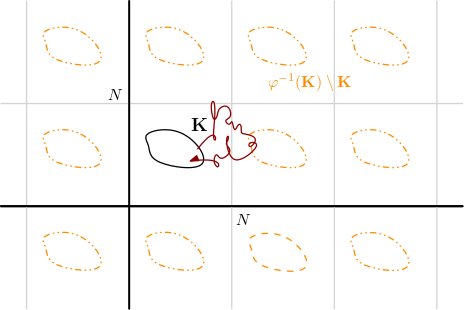
\includegraphics[width=0.72\columnwidth]{Figures/lattice shift.png}
    \caption{lattice shift of $K$ on $\mathbb{Z}_N^2$ and its inverse image}
    \label{lattice}
\end{figure}
\\From here, $\varphi(K)$ is denoted by $\mathbf{K}$ and $\varphi^{-1}$ is the inverse map from $\mathbb{Z}_N^d$ to $\mathbb{Z}^d$. To understand these two notations better, a simple example is illustrated here. 
As shown in Figure~\ref{lattice}, the black set represents $\varphi(K)$, and the orange sets represents $\varphi^{-1}(\mathbf{K})\setminus \mathbf{K}$. In addition, let $X_n$ be a SRW on $\mathbb{Z}^2$ that starts in $\partial_{int}\mathbf{K}$ and runs until time $n$ (the red trajectory in Figure~\ref{lattice}). Recall our definition of first hitting time $\Tilde{H}_A$, here $X_n$ is included in the set of events 
\begin{equation}
    \left\{X_n: \ \Tilde{H}_{\varphi^{-1}(\mathbf{K})\setminus \mathbf{K}} \leq n\right\}, \notag
\end{equation}
but does not belong to the set of events 
\begin{equation}
    \left\{X_n: \Tilde{H}_{\mathbf{K} } >n\right\} \setminus \left\{X_n: \Tilde{H}_{\varphi^{-1}(\mathbf{K})}>n \right\}. \notag
\end{equation}
\textit{Remark 4.3} Following this chapter, we also looked closely into the construction of random interlacements by a so called \textit{random interlacement point process}, based on the understanding of Poisson Point Processes (PPP). We think of random interlacements as a collection of double infinite trajectories being randomly put into a $\mathbb{Z}^d$, just as randomly dropping points into a space for PPP. Details of that process can be found in chapters 5 and 6 in \cite{drewitz2014introduction}.

\section{Cover Time of RW on Torus}
Finally, we look into a variation of the simple random walk, namely the so-called \textit{Elephant Random Walk} (ERW), involving some reinforcement due to a certain memory of the process, quantified by a memory parameter $p$ between $0$ and $1$. Based on \cite{comets2013large} and \cite{bercu2019multi}, we focus on the two-dimensions case and investigate the cover time of random walks and elephant random walks of a discrete torus $\mathbb{Z}_n^2$ and simulate RWs and ERWs on $\mathbb{Z}_n^2$ with different size of $n$ and $p$. Note that the behavior of random walks in two dimensions is generally different compared to their higher-dimensional counterparts due to its recurrence and strong correlation.
\subsection{Definitions and Asymptotic Results}
Introduced by Schütz and Trimper in \cite{schutz2004elephants}, the Elephant Random Walk in one dimension is a non-Markovian stochastic process referring to the saying that \textit{elephants can always remember where they have been}. Here we introduce ERWs in two dimensions. 
\vspace{0.6em}\\Let the random sequence $(X_n)_{n \geq 0}$ be a random walk on $\mathbb{Z}^2$. The random walk starts at some point $X_0 = x_0 \in \mathbb{Z}^2$ in time $t_0 = 0$. For the construction, we will use a sequence of i.i.d.~random variables $(\sigma_{t})_{t \geq 0}$, where  $\sigma_0$ takes values chosen uniformly at random from $\{(1,0), \ (-1,0), \ (0,1), \ (0,-1) \}$. At time $t_1$, the elephant chooses from the four directions to move forward: 
\begin{equation}
    X_1 = X_0 + \sigma_0, \ \sigma_0 \sim \mathscr{U}(\{(1,0), \ (-1,0), \ (0,1), \ (0,-1)\}). \tag{5.1}
\end{equation}    
For for the remaining steps $\left(X_{t+1}\right)_{t=1}^{n-1}$ up to time $n$, 
\begin{equation}
    X_{t+1}:=\left\{
\begin{aligned}
X_t + \sigma_i \quad &\text{ with probability } p,\\
X_t + \sigma_{t+1} \quad& \text{ with probability } 1-p,
\end{aligned}
\right.\tag{5.2}
\end{equation}
where $\sigma_{t+1} \sim \mathscr{U}(\{(1,0), \ (-1,0), \ (0,1), \ (0,-1)\})$, and $\sigma_i$ is chosen uniformly at random from $(\sigma_i)_0^t$. Following similar notation from section four, we use bold font to denote elephant random walks on the torus. 
\vspace{0.6em}\\An example of ERW $(\mathbf{X}_n)$ in two dimensions on a  discrete torus could look like Figure~\ref{2derw}(a). Here, the size of torus is set at $n=100$ and the walk runs for $5000$ steps. As a comparison, simple random walk (i.e. ERW with $p=0$) on $\mathbb{Z}^2_{100}$ is shown in Figure~\ref{2derw}(b).
\begin{figure}
    \centering
    \subfloat[ERW with $p=0.85$]{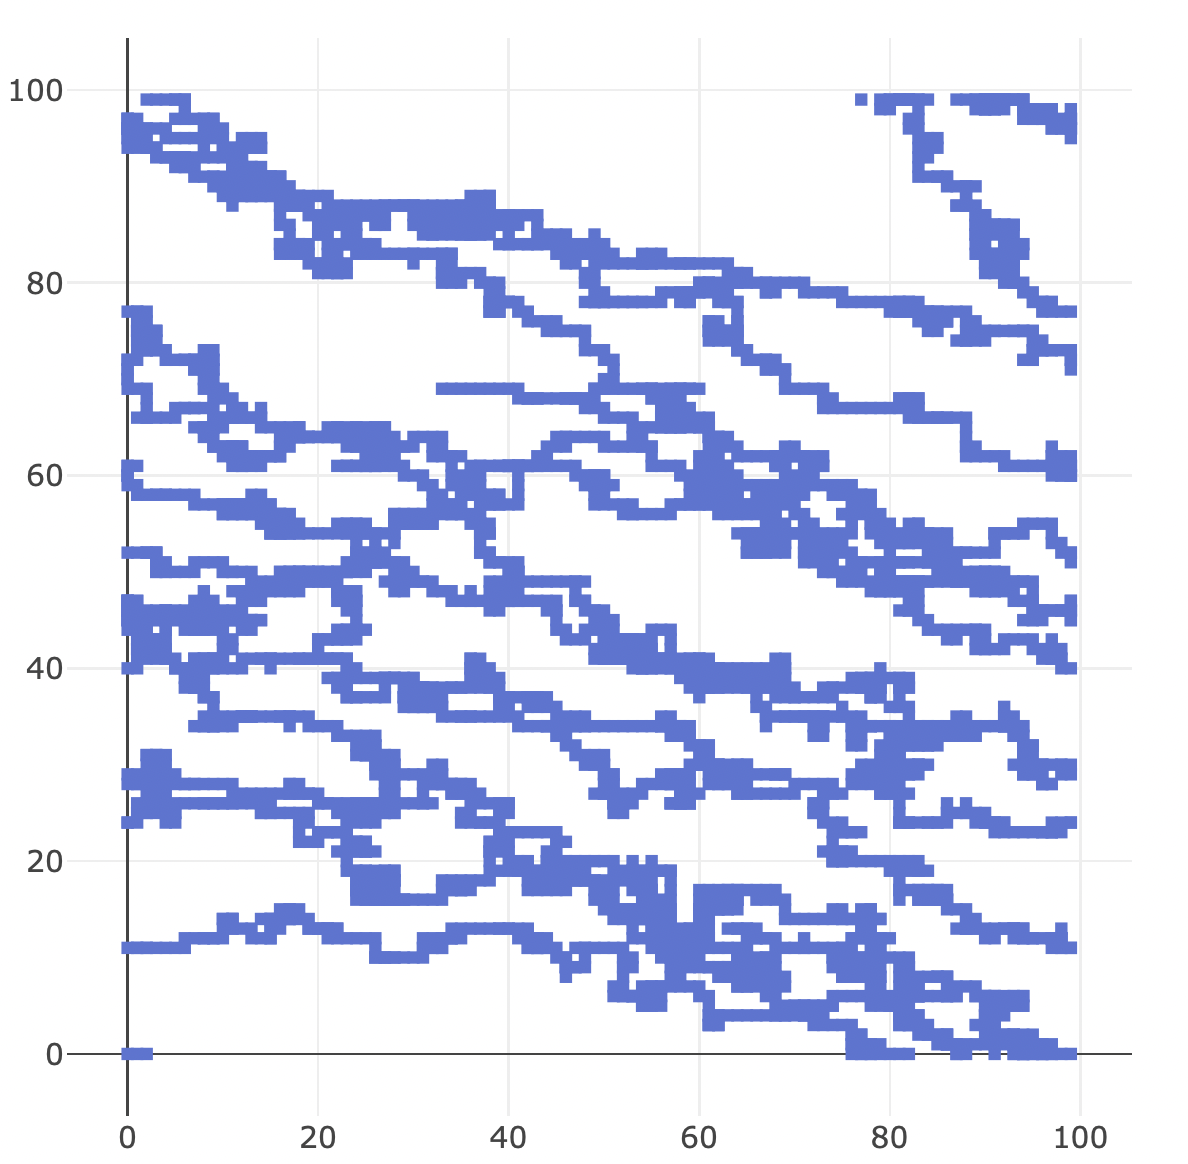
\includegraphics[width=.5\columnwidth]{Figures/EWR on 2d size 100 p=0.85.png}}
    \subfloat[SRW]{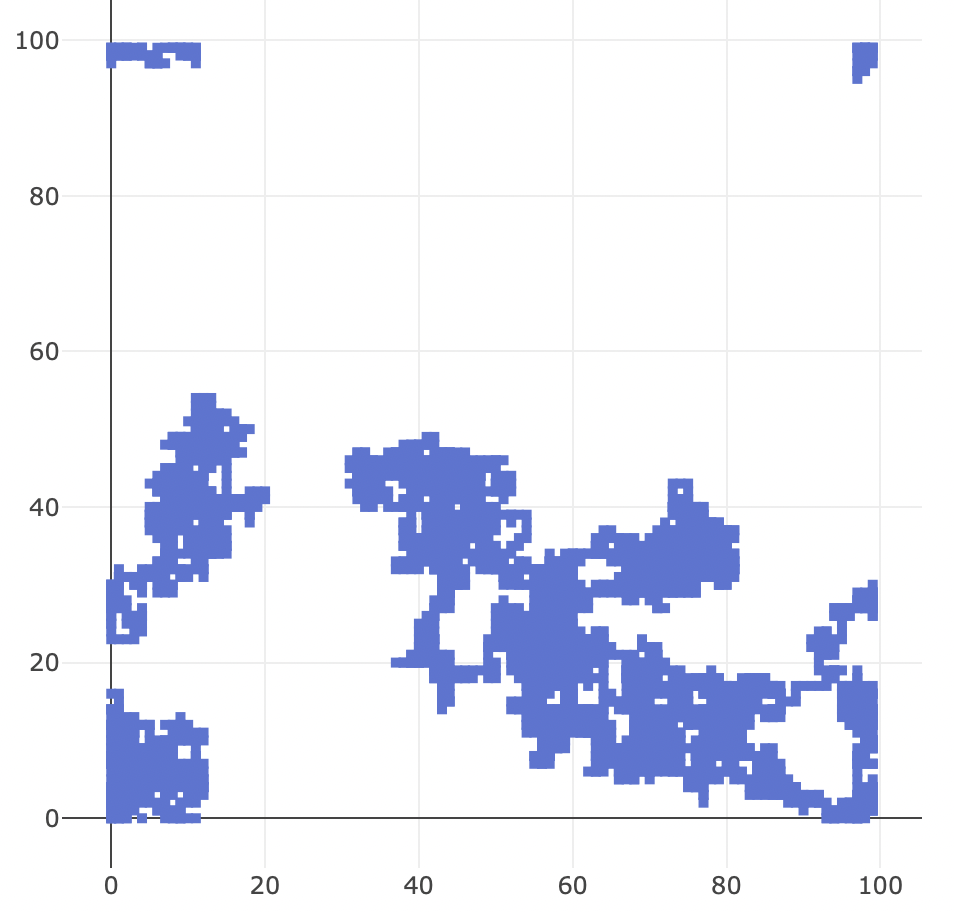
\includegraphics[width=.5\columnwidth]{Figures/2dSRW n=100.png}}
    \caption{Elephant random walk on $\mathbb{Z}_{100}^2$ when $p=0.85$ and $p=0$ in $5000$ steps} 
    \label{2derw}
\end{figure}
Results in \cite{bercu2019multi} shows that not only for ERW in dimension two, but for all multi-dimensional elephant random walks, the behavior of  the random walk changes markedly when the memory parameter $p$ reaches the critical value
\begin{equation}
    \label{eq5.3}
    p_d=\frac{2d+1}{4d}. \tag{5.3}
\end{equation}
As addressed in \eqref{eq5.3}, the critical $p$ in $\mathbb{Z}^2$ should be $0.625$. Depending on the value of $p$, ERWs can be can be categorized into diffusive ERWs, critical ERWs and superdiffusive ERWs.
\vspace{0.6em}\\\textbf{Definition 5.1} (diffusive, critical, superdiffusive) Let $(X_n)_{n \geq 0}$ be a multi-dimensional elephant random walk on the integer lattice $\mathbb{Z}^d$. We say that $(X_n)_{n \geq 0}$ is \textit{diffusive} if $p<p_d$, \textit{critical} if $p=p_d$, and \textit{superdiffusive} if $p>p_d$.
\vspace{0.6em}\\ Naturally, we are motivated to check the number of steps needed for an ERW to cover the whole torus. Such number of steps is called the cover time.
\vspace{0.6em}\\\textbf{Definition 5.2} (cover time) Let $(\mathbf{X}_n)_{n \geq 0}$ be a simple random walk, or elephant random walk on  $\mathbb{Z}_n^d$. The \textit{cover time} of the torus is 
\begin{equation}
    \mathcal{T}_n=\max_{\mathbf{x} \in \mathbb{Z}_n^d}H_\mathbf{x}(\mathbf{X}) \tag{5.4}
\end{equation}
where $H_x(\mathbf{X})$ denotes entrance time to the site ${\mathbf{x}}$ as we defined in \eqref{eq2.2}. By previous work in \cite{dembo2004cover}, it is proved that for $p = 0$ (i.e. for the simple random walk)
\begin{equation}
    \label{eq5.5}
    \frac{\mathcal{T}_n}{n^2\ln^2n}\xrightarrow[n \rightarrow \infty]{\mathbf{P}}\frac{4}{\pi}. \tag{5.5} 
\end{equation}
Generally there will be several last vacant points that take the ERW a long time to reach. Following in the literature after \cite{dembo2004cover}, such
\textit{late points} of random walks have also been studied. Deviations from the asymptotic value of the cover time have also been investigated for the simple random walk. A key insight is as follows: if one considers times that differ from the asymptotic value of the cover time by a constant factor in $(0,1)$, one can prove a stretched exponential decay in the corresponding torus size. This is formalized by large deviation lower bounds and upper bounds of the cover time, which are given by the following theorem, see~\cite{comets2013large}.
\vspace{0.6em}\\\textbf{Theorem 5.1} \textit{Assume that} $\gamma \in (0,1)$, \textit{then for all} $\varepsilon>0$, we have
\begin{equation}
    \exp{\left(-n^{2(1-\sqrt{\gamma})+\varepsilon}\right)} \leq \mathbf{P}\left[\mathcal{T}_n \leq \frac{4}{\pi}\gamma n^2\ln^2n \right] \leq \exp{\left(-n^{2(1-\sqrt{\gamma})-\varepsilon}\right)} \tag{5.6}
\end{equation}
\textit{for} $n$ \textit{large enough.}\vspace{0.6em}\\ 
In terms of upwards deviations from the asymptotic cover time, the following result (also due to~\cite{comets2013large}) is available.
\vspace{0.6em}\\\textbf{Theorem 5.2} \textit{Assume that} $\gamma>1$, \textit{then for all} $\varepsilon>0$, we have
\begin{equation}
    n^{-2(\gamma-1)-\varepsilon} \leq \mathbf{P}\left[\mathcal{T}_n \geq  \frac{4}{\pi}\gamma n^2\ln^2n \right] \leq n^{-2(\gamma-1)+\varepsilon} \tag{5.7}
\end{equation}
\textit{for} $n$ \textit{large enough.}
\vspace{0.6em}\\Additionally, for $\gamma \in (0,1)$, fix an arbitrary $\alpha \in (\sqrt{\gamma},1)$, consider simple random walk on the torus $\mathbb{Z}_n^2$ and divide the torus into boxes of size $n^\alpha$, there exists $c=c(\alpha,\gamma)>0$, \ $c'=c'(\alpha,\gamma)>0$ such that by time $t=\frac{4}{\pi}\gamma n^2\ln^2n$, there are at least $cn^{2(1-\alpha)}$ boxes not completely covered with probability at least 
\begin{equation}
    1-\exp\left(-c'n^{2(1-\alpha)}\right). \tag{5.8}
\end{equation}

\subsection{Implementation of SWR and EWR on $\mathbb{Z}_n^2$}
Surprisingly there is not much literature available about cover times of elephant random walks on $\mathbb{Z}_n^2$. Based on asymptotic results in section 5.1, we are motivated to simulate simple random walks and elephant random walks on $\mathbb{Z}_n^2$ to confirm the results in \cite{bercu2019multi} and construct a rough stretch for influence of memorization on the cover time for future investigation. 
\begin{figure}[htb]
    \centering
    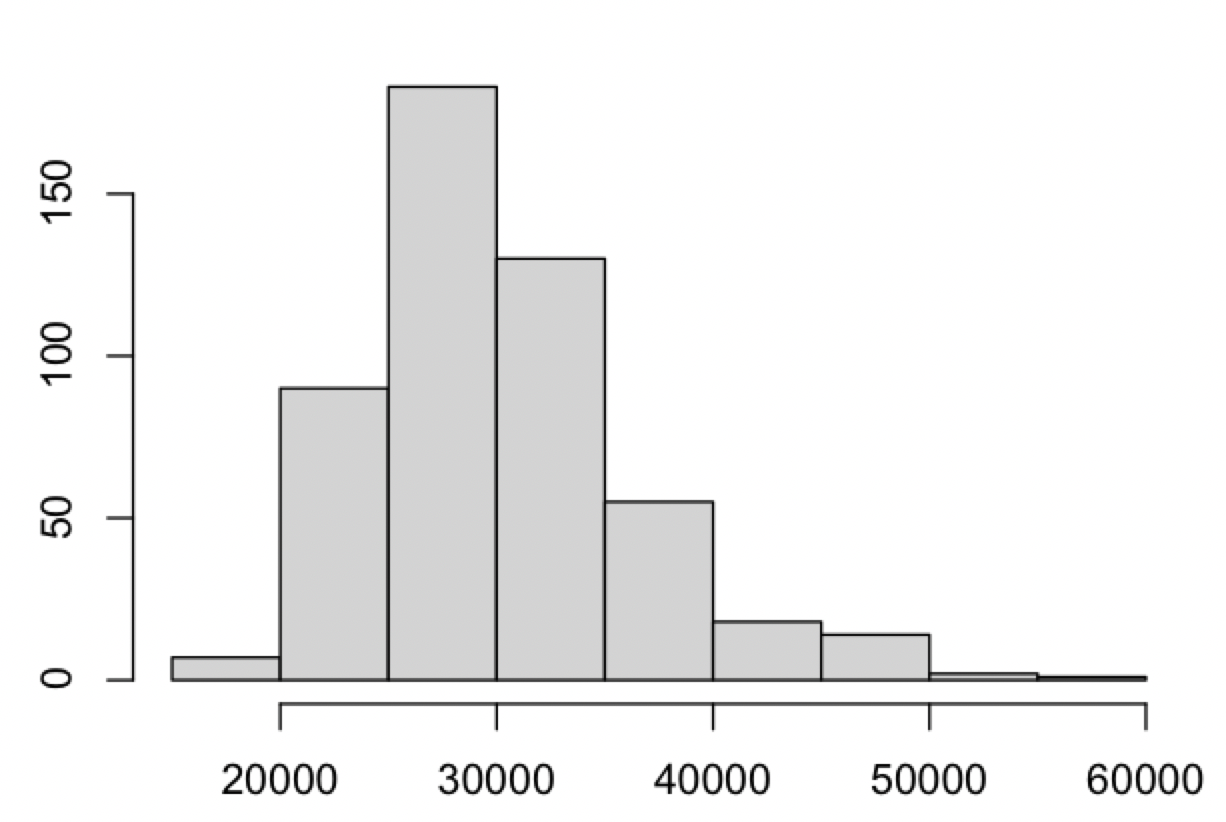
\includegraphics[width=.75\columnwidth]{Figures/redo p = 0 500.png}
    \caption{Histogram of cover time of simple random walk on $\mathbb{Z}_{50}^2$ for $500$ trials}
    \label{500}
\end{figure}
\vspace{0.6em}\\We start by simulating simple random walks on $\mathbb{Z}_n^2$, i.e. elephant random walks when $p=0$. We let the walk to run until it completely covers the torus, here of size $n=50$. We will simulate the random walk for $\mathcal{N} \in \mathbb{N}$ times (each run will be terminated until the entire torus is covered), and denote the corresponding walks by $(\mathbf{X}_t^{(j)})_{t \geq 0, j = 1,..., \mathcal{N}}$. Since $(\mathbf{X}_t^{(1)})_{t \geq 0},...,(\mathbf{X}_t^{(\mathcal{N})})_{t \geq 0}$ are i.i.d. random variables, by the Law of Large Numbers, the mean and median for the cover times should give us a nice picture of cover time of SRWs when we repeat for large number of times $\mathcal{N}$. According to our simulation, the mean cover time of a simple random walk on $\mathbb{Z}_{50}^2$ is around $30151.69$ and the median cover time is around $29045$, as the distribution is shown in Figure~\ref{500}. This result confirms the formula in \eqref{eq5.5}.
\vspace{0.6em}\\Now we vary the memory parameter $p$ and compare the cover time $\mathcal{T}_n$ at different $p$'s, as shown in Figure~\ref{5060} and Table~\ref{data}. 
\begin{figure}[h]
    \centering
    \subfloat[Torus Size $50$]{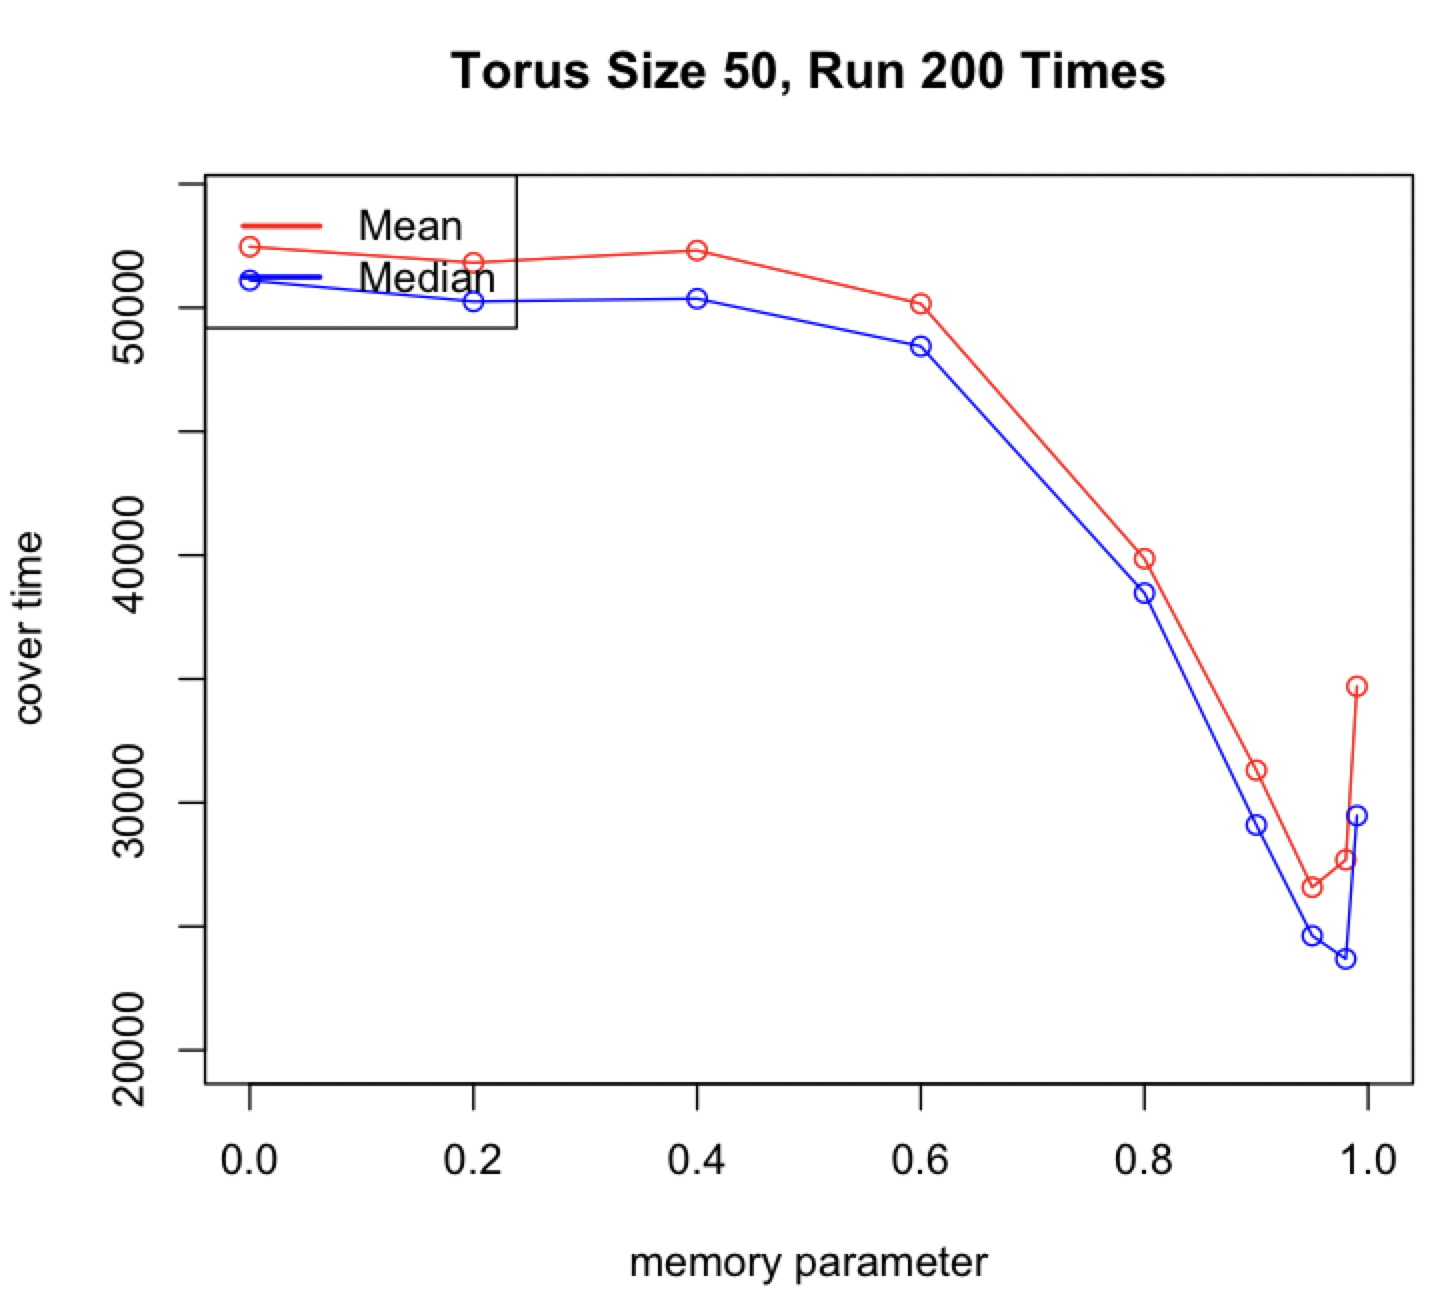
\includegraphics[width=.5\columnwidth]{Figures/t = 50 200 times.png}}
    \subfloat[Torus Size $60$]{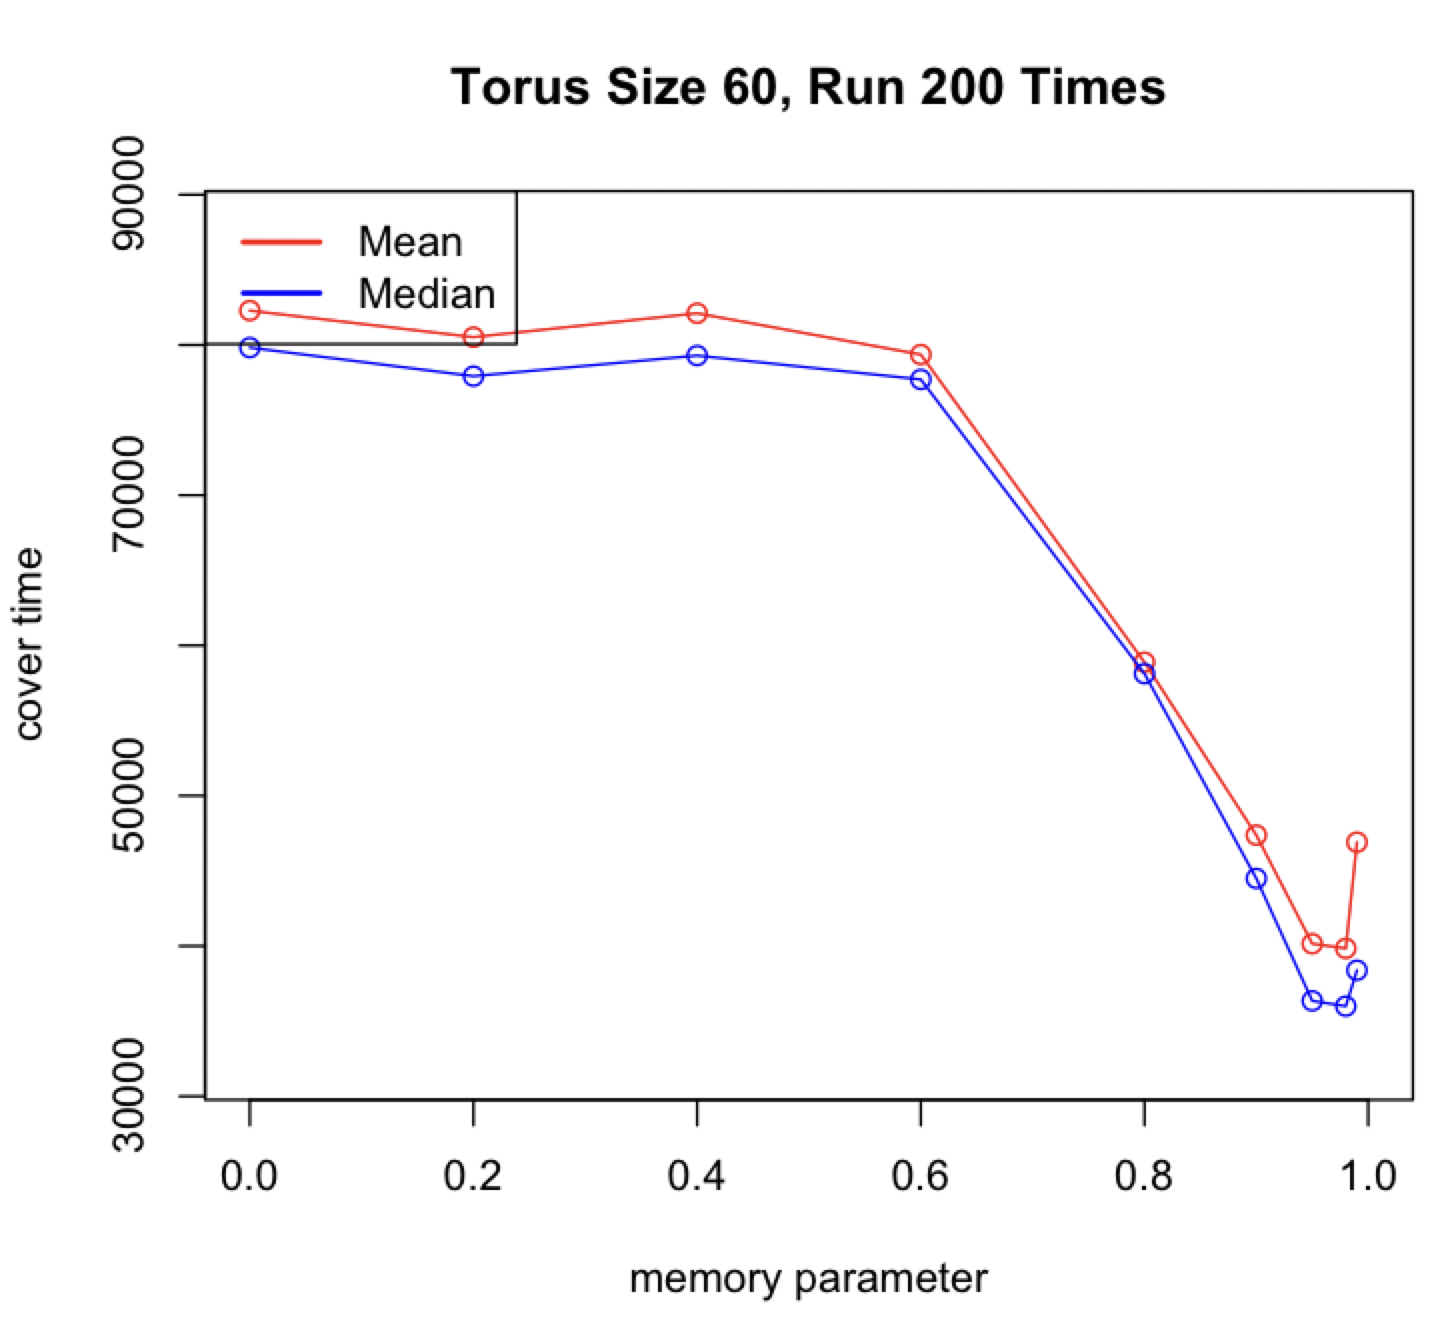
\includegraphics[width=.5\columnwidth]{Figures/t = 60 200 times.png}}
    \caption{Mean and median cover time with respect to memory parameter}
    \label{5060}
\end{figure}
\makeatletter
\setlength{\@fptop}{5pt}
\makeatother
\begin{table}
\caption{Mean and Median of Cover Time For Different Size of Torus}
\centering
\begin{tabular}{c|c|c|c|c|c|c}
\toprule
$p$ & \multicolumn{2}{|c|}{$40$} & \multicolumn{2}{|c|}{$50$}& \multicolumn{2}{|c}{$60$}\\
\midrule
\quad & mean & median & mean & median & mean & median\\
$0.00$ & $29768.52$ & $29525.0$ & $52465.99$ & $51106.2$ & $82285.32$ & $79824.2$\\
$0.20$ & $29929.55$ & $28622.1$ & $51818.55$ & $50251.1$ & $80517.99$ & $77921.7$\\
$0.40$ & $29494.57$ & $28791.5$ & $52312.52$ & $50366.5$ & $82109.38$ & $79294.2$\\
$0.60$ & $28593.09$ & $27929.2$ & $50162.05$ & $48443.2$ & $79361.77$ & $77705.6$\\
$0.80$ & $22590.21$ & $21435.1$ & $39860.43$ & $38470.5$ & $58882.81$ & $58125.5$\\
$0.90$ & $17935.65$ & $17198.5$ & $31312.68$ & $29100.8$ & $47377.38$ & $44495.5$\\
$0.95$ & $15601.31$ & $14544.6$ & $26583.77$ & $24624.7$ & $40153.21$ & $36350.2$\\
$0.98$ & $16063.24$ & $13887.2$ & $27693.42$ & $23689.5$ & $39840.40$ & $35996.0$\\
$0.99$ & $20680.24$ & $15751.9$ & $34702.23$ & $29478.5$ & $46909.86$ & $38386.5$\\
\bottomrule
\end{tabular}
\label{data}
\end{table}
For fixed torus size $n$, the cover time remains large when $p \leq p_d$ and it decreases as $p$ increases when $p \geq p_d$. In fact, it decreases to about half of the steps needed when $p=0$ as $p \rightarrow 1$. The curve finally had a steep increase around $p=1$, since the ERW with $p = 1$ can never cover the entire torus, $\mathcal{T}_n=\infty$.
\vspace{0.6em}\\From \eqref{eq5.5}, we know that $\mathcal{T}_n$ grows faster than quadratically when $n$ is large. Due to computational complexity, we only simulated ERWs up to $n=60$. No conclusions could yet been given, but a new conjecture could be that for ERWs with $p$ larger than critical value, there could be a lower bound for its cover time on $\mathbb{Z}_n^2$.



%----------------------------------------------------------------------------------------
%	BIBLIOGRAPHY
%----------------------------------------------------------------------------------------
\clearpage
\renewcommand{\refname}{\spacedlowsmallcaps{References}} % For modifying the bibliography heading

\bibliographystyle{unsrt}

\bibliography{sample.bib} % The file containing the bibliography

%----------------------------------------------------------------------------------------

\end{document}